\section{Likelihood of long-run frequencies}\label{sec:likelihood} 

%Claudia Examples with equally likely long-run freqs – we can have very different
%longrun MI leading to same sample MI. Introduced by a discrete example.
%Multinomial probabilities

In the previous section we showed that mutual information between the stimulus $s$ and the response $r$ computed directly from the sample may significantly vary across samples from the same population. In reality we don't typically have access to multiple samples, but we have to rely on one single sample to make an estimate of the population mutual information. As explained in section ... the population mutual information is a function of the population frequencies, or long-run frequencies, which are unknown. Yet we can use our data to inform us on the long-run frequencies that may have generated our sample and use them to estimate the population mutual information. How do we appraise candidate long-run frequencies for our data? Given the candidate long-run frequencies $\mathbf{f_s}=\{f_s(r)\}_{s,r}$ and a sample $\hat{s}$, the likelihood of these long-run frequencies $P(\hat{s}\vert \mathbf{f_s})$ is the probability that our sample was generated from a population with such long-run frequencies. For the dataset of spike-count responses and north/south head direction stimulus introduced in section ... the likelihood of long-run frequencies $\mathbf{f_s}$ is: 


\begin{equation}
P(\hat{s}\vert \mathbf{f_s})=\prod_{s,r} f_s(r)^{N\hat{f}_s(r)}
%\frac{N!}{\prod_{s,r} \hat{f}_s(r)!}\prod_{s,r} f_s(r)^{N\hat{f}_s(r)}
\label{eq:categorical_likelihood}
\end{equation}

where $\hat{f}_s(r)$ are the sample frequencies shown in Fig.~\ref{fig:sample_frequencies}. 

It can be easily seen that the long-run frequencies that maximize the likelihood in Eq. \ref{eq:categorical_likelihood} are the sample frequencies $f_s(r)=\hat{f}_s(r)$. Thus, in order to estimate the population mutual information between head direction and spike count, it might be tempting to simply compute the mutual information from the sample frequencies being the maximum-likelihood ones, while disregarding other potential long-run frequencies. Such point estimator of the population mutual information has indeed the convenient property of being asymptotically optimal, meaning that for infinite data size, the maximum likelihood estimator converges to the population one \textcolor{red}{Ref}. 

In real experiments the data sample size is always limited, which is why the maximum-likelihood estimator can be a poor estimator in practice. Several authors \textcolor{red}{Refs} have indeed pointed out that the maximum-likelihood estimate of the mutual information can be biased, because of the very nature of the mutual information being positively defined. Beyond its bias the one-shot maximum-likelihood estimation is problematic in many ways. 
Ultimately the main (and fixable!) issue is that it's limited to a single candidate long-run frequency, while either previous knowledge about the system, or the likelihood itself, might indicate that other long-run frequencies should be considered. In the next two subsections we illustrate this point by considering the three long-run frequencies in Fig. \ref{fig:highlike_long-run_freqs} for the sample $\hat{s}$, introduced in section ..., from which we want to estimate the population mutual information between head direction and spike count.

%But the maximum-likelihood mutual information is point estimator and as such it does not incorporate a measure of the uncertainty associated to such estimate. Intuitively one realizes that by choosing the maximum-likelihood frequencies and computing the mutual information from them, one disregards the actual value of the likelihood.  Such value might be instead exploited to express our degree of belief (and uncertainty) on our mutual information estimate, as inherited from the degree of belief on the long-run frequencies. We will elaborate on how in the next sections.

%In the previous section we introduced the definition of Mutual Information between stimulus and responses (some measure/parametrization of neural activity), as a function of the long-run conditional frequencies of the responses on the stimulus. Unfortunately, for any biological neural system, the long-run frequencies are unknown, while what we have at our disposal is typically a limited\footnote{limited is a vague word. In this work we consider a sample limited if the number of datapoints is of the same order of magnitude of the possible combinations of stimulus and response value.} sample drawn from these unknown long-run frequencies. In order to compute the mutual information between stimulus and response, we hence want to use our data to make a guess of the long-run frequencies. How can we tell which long-run frequencies would most likely have generated our data? Let's think at the problem in reverse: if we knew the long-run frequencies then the likelihood $P(\hat{s}\vert \mathbf{f_s})$ would tell us how likely is our sample. It follows that for in the case of unknown long-run frequencies, the likelihood of \textit{candidate} long-run frequencies for our data can instruct us on how likely they might have generated the sample. How to choose the candidate long-run frequencies though? And, should be the likelihood the only metric for appraising long-run frequencies? One might be tempted to chose as a candidate only the long-run frequencies that maximize the likelihood for our data, namely the sample frequencies. Let's see why this problematic for a limited sample:

\subsection*{High-likelihood long-run frequencies beyond the maximum-likelihood ones}
By choosing the maximum likelihood estimator of the population frequencies and computing the mutual information just from it, one disregards completely other long-run frequencies which might have only a slightly smaller likelihood. 

As an example consider the three candidate long run frequencies for the sample $\hat{s}$ in sec... displayed in Fig.\ref{fig:highlike_long-run_freqs}. They look pretty similar and all have log-likelihoods which deviates less then $10\%$ from the maximum of the log-likelihood. Although these long-run frequencies might have generated our data with similar probability (likelihood), they yield rather different values of mutual information between spike count and head direction ( MIs up to $50\%$ apart). The examples in Fig.\ref{fig:highlike_long-run_freqs} therefore suggest that the maximum-likelihood mutual information (bottom of Fig.\ref{fig:highlike_long-run_freqs}) alone  might be poorly representative of the spectrum of mutual information values corresponding to high-likelihood long-run frequencies. As a consequence, we argue that a logical approach to mutual information estimation must encompass a range of long-run frequencies, while taking into account their likelihood. 


\subsection*{Maximum-likelihhod estimates disregard prior information} 

By choosing the maximum-likelihood frequencies as the only candidate long-run frequencies for our data, one approaches the sample in a completely \textcolor{red}{agnostic fashion}.
\mynote{This sounds like a positive thing: more focus on it actually being a strong assumption.} 



The assumption made by maximum-likelihood estimation is indeed that the researcher doesn't have any kind of pre-sample knowledge about the biologically plausible candidate long-run frequencies, or in other words, that the system of interest could in principle attain any population frequency with equal probability, until the sample is collected. 
Such an assumption is typically wrong, as:

\begin{enumerate}

\item \textbf{the very same neural system might have been probed before}, providing us evidence in favor of some candidate long-run frequencies over others. Suppose for example that, before collecting our sample $\hat{s}$ in fig ... , we had recorded the activity of the same neuron, while the animal was exploring the same environment. Suppose that from this recording we estimated a population mutual information between spike count and head direction of $0.1$ (an its associated uncertainty). When we now are about to collect the new sample $\hat{s}$ in fig ..., we don't just want to disregard this previous information on the system and regard every frequency as a priori equally good candidate for generating the new sample. We would rather consider the long-run frequency at the top of Fig. \ref{fig:highlike_long-run_freqs} as a better candidate than the one at the bottom of Fig. \ref{fig:highlike_long-run_freqs}, since the latter corresponds to a much higher mutual information. 

\item \textbf{the neural system of interest might have been investigated before and its results reported in the literature}. For our example of spike count vs head direction, we might know that the region we are recording from is characterized by bursty neurons with low, but different from zero, baseline firing rate. A-priori we would therefore assign a larger probability to the long-run frequency in the middle of Fig. \ref{fig:highlike_long-run_freqs} than to those at the bottom of Fig. \ref{fig:highlike_long-run_freqs}, for which the neuron is always silent in one of the two head-direction conditions.  

\item \textbf{biological constraints on the long-run frequencies for the system under investigation might be well established}. Assigning equal probability to every long-run frequency means that before conducting our experiment we regard long-run frequencies which are not attainable by the system of interest on equal footing with those actually attainable. In our example, where the response variable is the spike count, we know that a long-run frequency corresponding to an average firing rate larger than $500$Hz violates physiological constraints on the neural activity. Intuitively we want to assign such long-run frequencies very low, if not zero, a priori probability.

\end{enumerate}

Once the sample $\hat{s}$ is collected  and attributes maximum likelihood to the long-run frequency at the bottom of Fig. \ref{fig:highlike_long-run_freqs}, we intuitively want to combine this new information on long-run frequencies provided by the likelihood, with the old (prior) piece of information about the system. Disregarding prior information would simply be poor practice.

\vspace{1cm}
In this section we explained why considering only one long-run frequency, even if it's the log-likelihood one with its nice asymptotic convergence to the truth, may be reductive for the purpose of estimating the mutual information.
So if a single estimator of the mutual information based on solely the likelihood of the long-run frequencies is not a good estimator of the mutual info: how to construct a better one by encompassing a range of candidate long-run frequencies and incorporating prior knowledge on the system? We answer to this question in section ..., whereas in section ... we elaborate on how to formally express prior knowledge about the system.

\begin{figure}
\centering
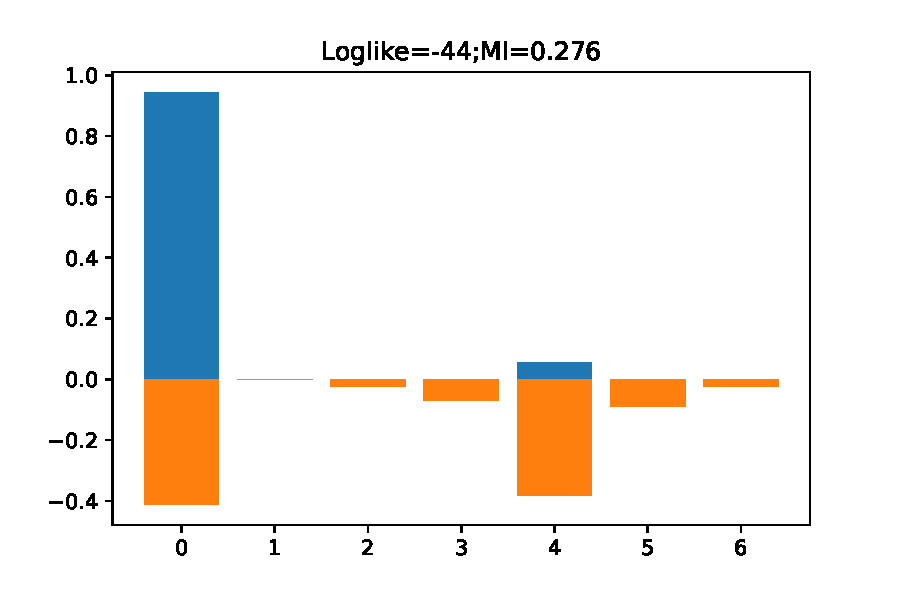
\includegraphics[scale=0.5]{HighLike_Plots1.pdf}\\ 
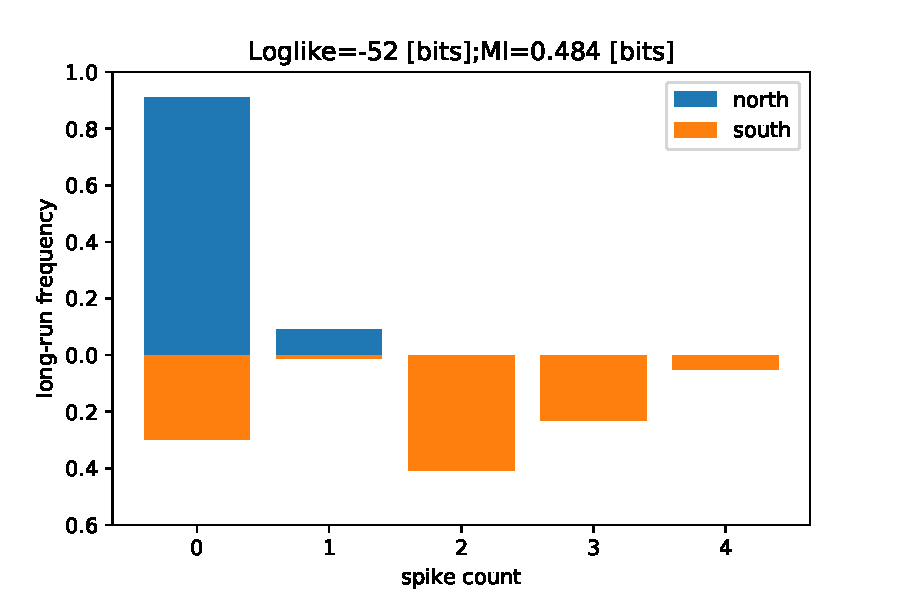
\includegraphics[scale=0.5]{HighLike_Plots0.pdf}\\
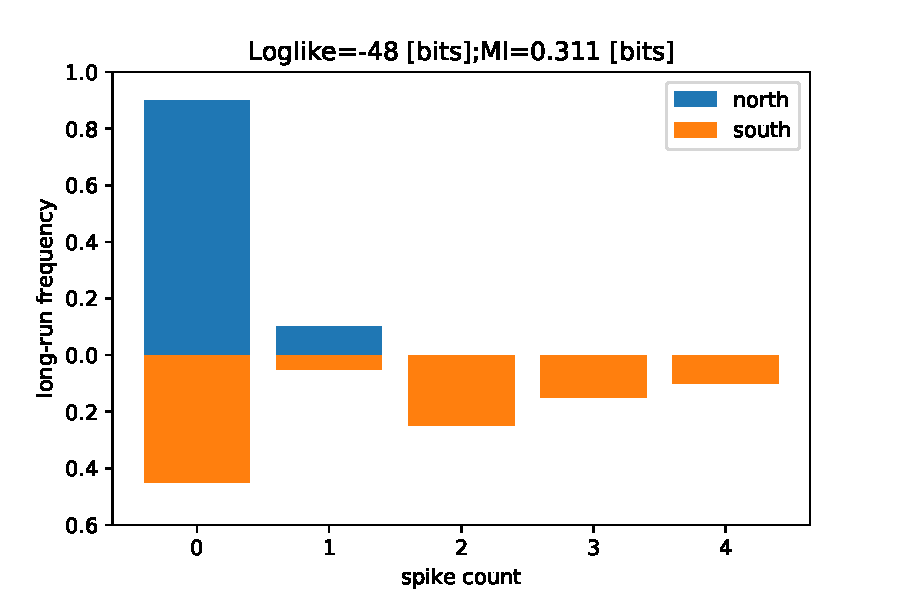
\includegraphics[scale=0.5]{HighLike_Plots_MaxLike.pdf} 
\label{fig:highlike_long-run_freqs}
\caption{High likelihood long-run frequencies for the data in sec. \ref{example1}. Examples of high likelihood long-run frequencies corresponding to low MI (top), medium MI (center), high MI and maximum likelihood (bottom). }
\end{figure}

\mynote{Plot long-run frequencies of other cells in the same dataset and average across cells.}